\documentclass[12pt]{exam}



\usepackage{graphicx}% Include figure files
\usepackage{dcolumn}% Align table columns on decimal point
\usepackage{bm}% bold math
\usepackage{latexsym}
\usepackage{amsmath,amssymb,amsthm,amsfonts}
\usepackage{subfigure}

\begin{document}
\pagestyle{head} \extraheadheight{1in}\runningheadrule
\firstpageheader{$\mbox{}$\\DATE: March 7, 2007\\PAPER NO.: - \\
DEPARTMENT $\&$ COURSE NO.: MATH 3530\\EXAMINATION: Mathematical Problems in Biology  }{\bf UNIVERSITY OF MANITOBA\\
$\mbox{}$
\\$\mbox{}$ \\ $\mbox{}$\\$\mbox{}$}{$\mbox{}$\\Test 1\\ PAGE NO.: \thepage\ of \numpages\\TIME: 90
minutes\\ EXAMINER: S. Portet}\runningheadrule
\runningheader{$\mbox{}$\\DATE: March 7, 2007\\PAPER NO.: - \\
DEPARTMENT $\&$ COURSE NO.: MATH 3530\\EXAMINATION: Mathematical Problems in Biology }{\bf UNIVERSITY OF MANITOBA\\
$\mbox{}$
\\$\mbox{}$ \\ $\mbox{}$\\$\mbox{}$}{$\mbox{}$\\Test 1\\ PAGE NO.: \thepage\ of \numpages\\TIME: 90
minutes\\ EXAMINER: S. Portet} \vspace{-2.5cm}
\begin{center}
\begin{tabular}{cp{15.5cm}}
\hline
&\\
\end{tabular}
\end{center}
%\footer{}{Page \thepage\ of \numpages}%
%{\iflastpage{End of exam.}{Please go on to the next page\ldots}}

\addpoints


\vspace{0.1in} \hbox to \textwidth{NAME:\enspace\hrulefill}
\vspace{0.2in} \hbox to \textwidth{STUDENT NUMBER:\enspace\hrulefill
 SEAT NUMBER:\enspace\hrulefill} \vspace{0.2in} \hbox to
\textwidth{SIGNATURE:\enspace\hrulefill}

\vspace{.5in}

This is a 90 minute exam. Lecture Notes are allowed.

\vspace{.2in} This exam has 6 questions.

\vspace{.2in} {\bf \Large PLEASE SHOW YOUR WORK CLEARLY.} A correct answer without explanation will not get full marks. \vspace{.5in}
\begin{center}
\gradetable[v]
\end{center}



\newpage



\begin{questions}
\question[15]
Consider a species that lives for two years and may reproduce at the end of year one or
year two. 
\begin{itemize}
\item the mean number of offspring that 0-year olds have the following year is 1
\item the mean number of offspring that 1-year olds have the following year is 4
\item the probability that a 0-year old survives to be a 1-year old is 0.1.
\end{itemize}
\begin{parts}
\part Set up the Leslie matrix model.
\part Assume that the initial population consists of ten 0-year olds and six 1-year olds. How
many 0-year olds and how many 1-year olds will there be one year later.
\part Find the growth rate and the stable age distribution.\newpage
\end{parts}


\question[8]
The dynamics of a particular population (measured in thousand) of birds is described as follows
$$\frac{dP}{dt}=4P(1-8P^3)$$
\begin{parts}
\part Find the equilibria.
\part Determine the local stability of each equilibrium.
\end{parts}
\newpage

\question[8]
The population (measured in billions) of insects in generation $t$ is described as follows
$$P_{t+1}=P_t e^{4(1-3P_t)}$$
\begin{parts}
\part Find all equilibria.
\part Determine the local stability of each equilibrium.
\end{parts}
\newpage

\question[8]
Consider the difference equation that represents the size of a population in generation $t+1$ 
$$x_{t+1}=f(x_t),$$
its graph is shown in the Figure below
\begin{center}
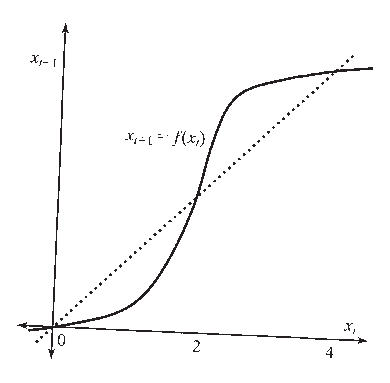
\includegraphics[width=.9\textwidth,,angle=2]{FigureTest1}
\end{center}
\begin{parts}
\part Find all equilibria. 
\part Determine the local stability of each equilibrium.
\end{parts}
\newpage


%\question[6]
%Show that the $2-$cycle
%$$\bar x_{1,2}=\frac{1\pm \sqrt{4r-3}}{2}$$
%of the difference equation $x_{t+1}=r-x_t^2$ is unstable if $r> 5/4$.
%\newpage


\question[6]
Show that 
$$ x_{t+1}=\frac{ax_t}{b +x_t}, \quad a,b>0$$
has no $2-$cycle.
\newpage





\question[15]
Show that the two-dimensional system
$$
\begin{array}{ll}
x_{t+1}=&x_{t}(1+x_{t}+y_{t})/3\\
y_{t+1}=&y_{t}(1-x_{t}+y_{t})/2
\end{array}
$$
has four fixed points, but only one that is locally stable.
\newpage
\mbox
%Consider the differential equation: $\frac{dy}{dx}=y^2-4$ (Do not
%solve the equation)
%\begin{enumerate}
%\item Is the above differential equation linear or nonlinear,
%autonomous or non-autonomous? Explain.
%\item Find the equilibrium solutions.
%\item Among the 3 direction fields shown on the next page, select
%the one corresponding to the above differential equation.
%\item Use the appropriate direction field to draw an approximate
%integral curve that satisfies $y(0)=0$.
%\item  What is the behavior of your solution in part 4 as $x$ goes
%to $+\infty$; in other words what is $\lim \limits_{x\rightarrow
%\infty}y(x)$?
%\end{enumerate}
%\begin{figure}[ht]
%\centering \subfigure[]{
%\includegraphics[width=.49\textwidth]{Figure1}}
%\subfigure[]{
%\includegraphics[width=.49\textwidth]{Figure2}}
%\subfigure[]{
%\includegraphics[width=.49\textwidth]{Figure3}}
%\end{figure}



%\section*{Question 2} \marginpar{[11]}
%Consider the differential equation: $x\frac{dy}{dx}+y=x^2$
%\begin{enumerate}
%\item Find the general solution of the above differential equation.
%\item What is the interval of validity of solutions?
%\end{enumerate}


%\section*{Exercise 3}
%Consider the differential equation: $\frac{dy}{dt}=ty+t$
%\begin{enumerate}
%\item Show that $y=-1$ is a solution of the above differential equation.
%\item Find the general solution of the above differential equation.
%\end{enumerate}

%\section*{Question 3}\marginpar{[14]}
%Consider the differential equation:
%$\frac{dy}{dx}=-\frac{1}{2}xy^3(1+x^2)^{-1/2}$
%\begin{enumerate}
%\item Show that $y(x)=0$ is a solution of the above differential equation.
%\item Find the general solution of the above differential equation.
%\item Find the solution that satisfies $y(0)=1$.
%\end{enumerate}

%\newpage
%\section*{Question 4}\marginpar{[11]}
%A population of butterflies in a forest increases at a rate $r$
%proportional to the total population. Initially, there are $20,000$
%butterflies, and birds eat $1,000$ butterflies per days.
%\begin{enumerate}
%\item Construct a mathematical model (\emph{i.e.}, differential equation and initial condition) to determine the population of
%butterflies in the forest at any time. Explain your variables,
%parameters and the units used. (Do not solve the equation)
%\item In the
%absence of predators (\emph{i.e.}, with no birds), biologists
%observe that the population triples each week. Calculate the rate of
%birth $r$ of butterflies in the forest (leave your answer with
%logarithms).
%\end{enumerate}




\end{questions}
\end{document}
